\newcommand{\OPT}[1]{\texttt{#1}}
\newcommand{\OPTprintValidExecutionTraces}{-\,-print-Execution-Traces}
\newcommand{\OPTprintInvalidExecutionTraces}{-\,-print-invalid-Execution-Traces}
\newcommand{\OPTprintMessageTraces}{-\,-print-Message-Traces}
\newcommand{\OPTprintDeploymentEquivalenceClasses}{-\,-print-Deployment-Equivalence-Classes}
\newcommand{\OPTprintAssemblyEquivalenceClasses}{-\,-print-Assembly-Equivalence-Classes}
\newcommand{\OPTplotDeploymentSequenceDiagrams}{-\,-plot-Deployment-Sequence-Diagrams}
\newcommand{\OPTplotAssemblySequenceDiagrams}{-\,-plot-Assembly-Sequence-Diagrams}
\newcommand{\OPTplotCallTrees}{-\,-plotCallTrees}
\newcommand{\OPTplotAggregatedDeploymentCallTree}{-\,-plot-Aggregated-Deployment-Call-Tree}
\newcommand{\OPTplotAggregatedAssemblyCallTree}{-\,-plot-Aggregated-Assembly-Call-Tree}

\newcommand{\OPTplotContainerDependencyGraph}{-\,-plot-Container-Dependency-Graph}
\newcommand{\OPTplotDeploymentComponentDependencyGraph}{-\,-plot-Deployment-Component-Dependency-Graph}
\newcommand{\OPTplotAssemblyComponentDependencyGraph}{-\,-plot-Assembly-Component-Dependency-Graph}
\newcommand{\OPTplotDeploymentOperationDependencyGraph}{-\,-plot-Deployment-Operation-Dependency-Graph}
\newcommand{\OPTplotAssemblyOperationDependencyGraph}{-\,-plot-Assembly-Operation-Dependency-Graph}

\section{Execution Traces, Message Traces, and Trace Equivalence Classes}

\subsection{Execution Traces}\label{sec:example:executionTraces}%

Textual execution trace representations of valid/invalid traces are written to %
an output file using the command-line options \OPT{\OPTprintValidExecutionTraces} and %
\OPT{\OPTprintInvalidExecutionTraces}. %
Listing~\ref{lst:appendix:traceAnalysisExample:executionTraces} %
shows the execution trace representation for the valid trace \ldots6129.

\setTextListing
\lstinputlisting[firstline=1,lastline=5,escapechar={},%
caption=Textual output of trace 6488138950668976129's execution trace representation,%
label=lst:appendix:traceAnalysisExample:executionTraces]%
{images/example-plots/executionTraces.txt}

\subsection{Message Traces}\label{sec:example:messageTraces}%

Textual message trace representations of valid traces are written to an output %
file using the command-line option \OPT{\OPTprintMessageTraces}. %
Listing~\ref{lst:appendix:traceAnalysisExample:messageTraces} %
shows the message trace representation for the valid trace \ldots6129.

\setTextListing
\lstinputlisting[firstline=1,lastline=9,escapechar={},%
caption=Textual output of trace 6488138950668976129's message trace representation,%
label=lst:appendix:traceAnalysisExample:messageTraces]%
{images/example-plots/messageTraces.txt}

\subsection{Trace Equivalence Classes}\label{sec:example:traceEquivClasses}%

Deployment/assembly-level trace equivalence classes are computed and written %
to output files using the command-line options \OPT{\OPTprintDeploymentEquivalenceClasses} %
and \OPT{\OPTprintAssemblyEquivalenceClasses}. %
Listings~\ref{lst:appendix:traceAnalysisExample:traceDeploymentEquivClasses} and %
\ref{lst:appendix:traceAnalysisExample:traceAssemblyEquivClasses} show the %
output generated for the monitoring data used in this section. %

\setTextListing
\lstinputlisting[caption=Textual output of information on the \textit{deployment-level} trace equivalence classes,%
label=lst:appendix:traceAnalysisExample:traceDeploymentEquivClasses]
{images/example-plots/traceDeploymentEquivClasses.txt}

\setTextListing
\lstinputlisting[caption=Textual output of information on the \textit{assembly-level} trace equivalence classes,%
label=lst:appendix:traceAnalysisExample:traceAssemblyEquivClasses]%
{images/example-plots/traceAssemblyEquivClasses.txt}

\section{Sequence Diagrams}\label{sec:example:seqDiagrams}%

\subsection{Deployment-Level Sequence Diagrams}\label{sec:example:deploymentSeqDiagrams}%

Deployment-level sequence diagrams are generated using the command-line option \OPT{\OPTplotDeploymentSequenceDiagrams}. %
Figures~\ref{fig:appendix:traceAnalysisExample:SeqDiagrsDepl6129}--\ref{fig:appendix:traceAnalysisExample:SeqDiagrsDepl6141} %
show these sequence diagrams for each deployment-level %
trace equivalence representative (Section~\ref{sec:example:traceEquivClasses}).

\begin{figure}[h]\centering
\subfigure[Trace \ldots{}6129]{\label{fig:appendix:traceAnalysisExample:SeqDiagrsDepl6129}%
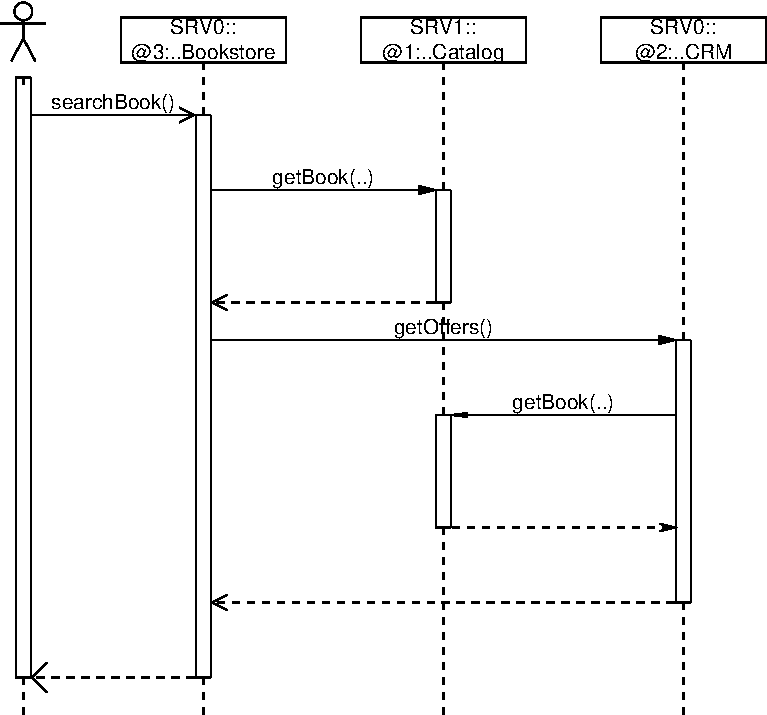
\includegraphics[scale=0.4]{images/example-plots/deploymentSequenceDiagram-6488138950668976129-crop}
}
\subfigure[Trace \ldots{}6130]{\label{fig:appendix:traceAnalysisExample:SeqDiagrsDepl6130}%
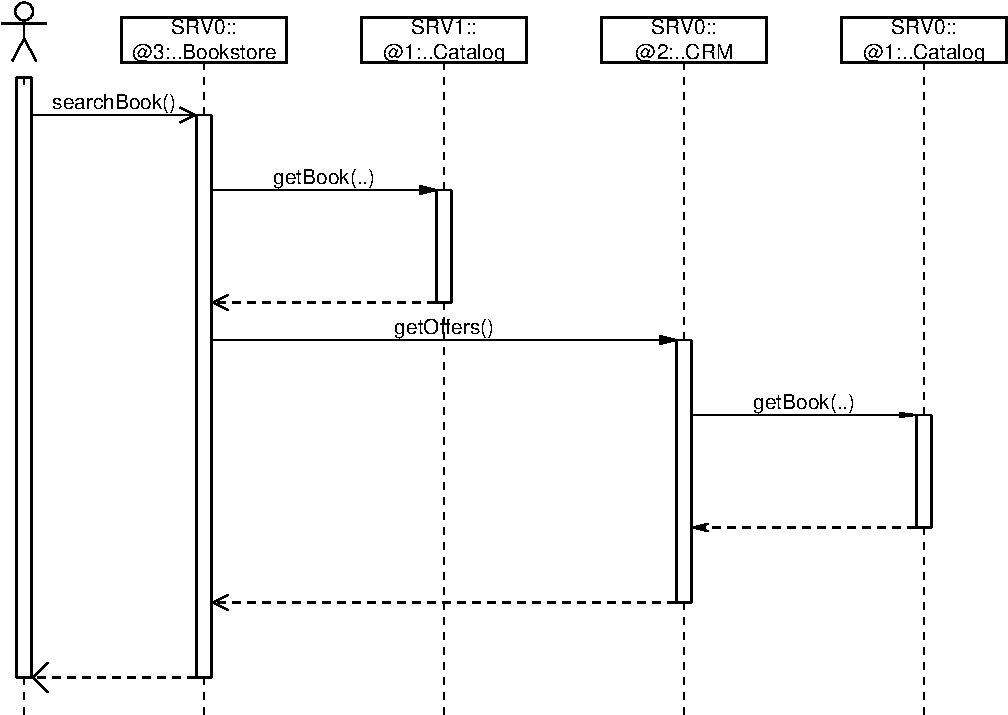
\includegraphics[scale=0.4]{images/example-plots/deploymentSequenceDiagram-6488138950668976130-crop}
}
\subfigure[Trace \ldots{}6131]{\label{fig:appendix:traceAnalysisExample:SeqDiagrsDepl6131}%
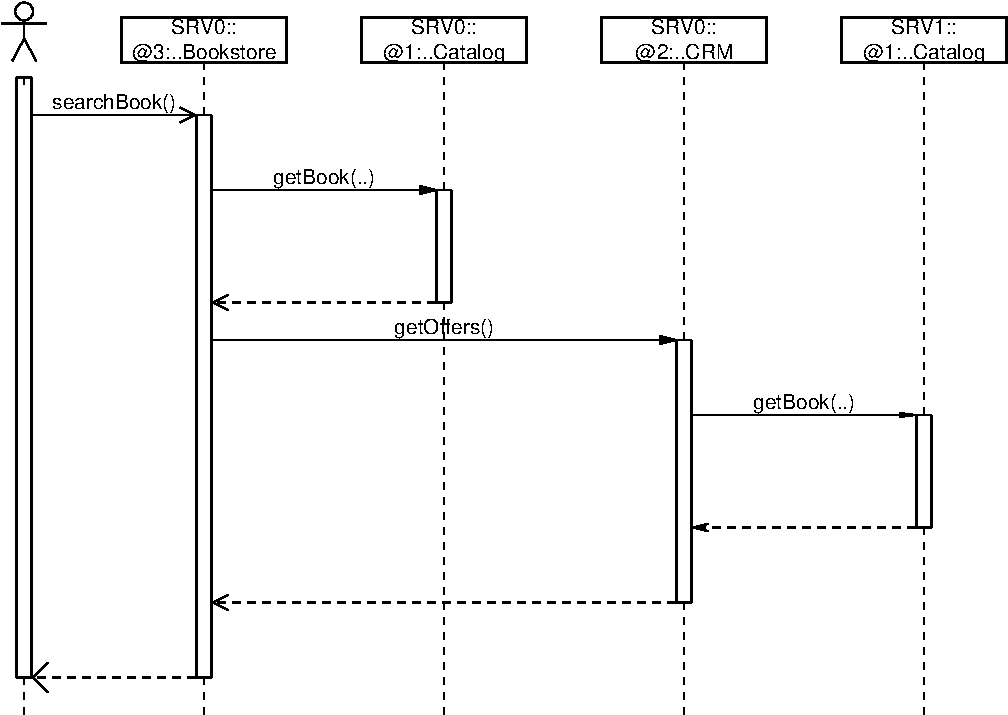
\includegraphics[scale=0.4]{images/example-plots/deploymentSequenceDiagram-6488138950668976131-crop}
}
\subfigure[Trace \ldots{}6141]{\label{fig:appendix:traceAnalysisExample:SeqDiagrsDepl6141}%
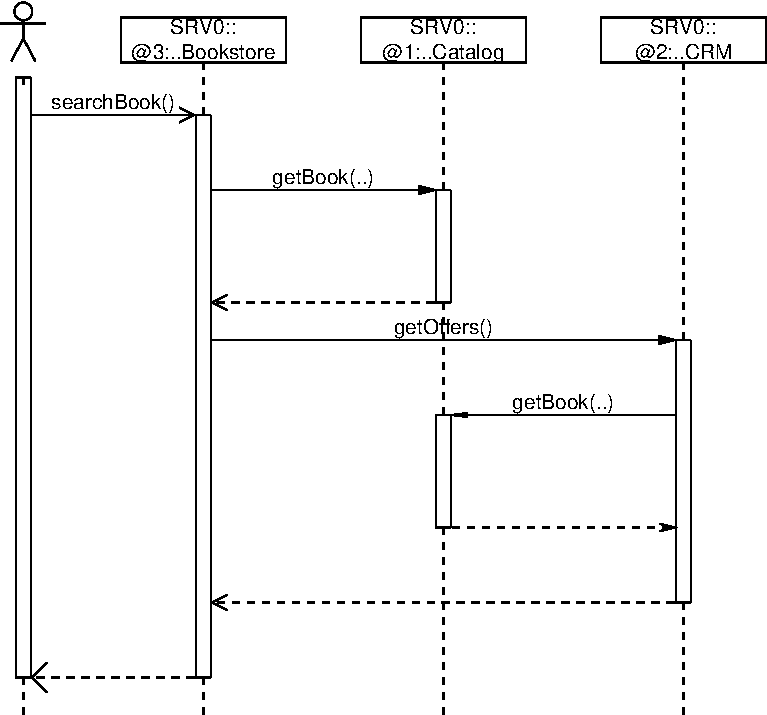
\includegraphics[scale=0.4]{images/example-plots/deploymentSequenceDiagram-6488138950668976141-crop}
}
\caption{\textit{Deployment-level} sequence diagrams of the trace %
equivalence class representatives (Listing~\ref{lst:appendix:traceAnalysisExample:traceAssemblyEquivClasses})}
\label{fig:appendix:traceAnalysisExample:SeqDiagrsDepl}
\end{figure}

\subsection{Assembly-Level Sequence Diagrams}\label{sec:example:assemblySeqDiagrams}%

Assembly-level sequence diagrams are generated using the command-line option \OPT{\OPTplotAssemblySequenceDiagrams}. %
Figure~\ref{fig:appendix:traceAnalysisExample:SeqDiagrDepl6129} %
show the sequence diagram for the assembly-level trace equivalence representative %
(Section~\ref{sec:example:traceEquivClasses}).

\begin{figure}[h]\centering
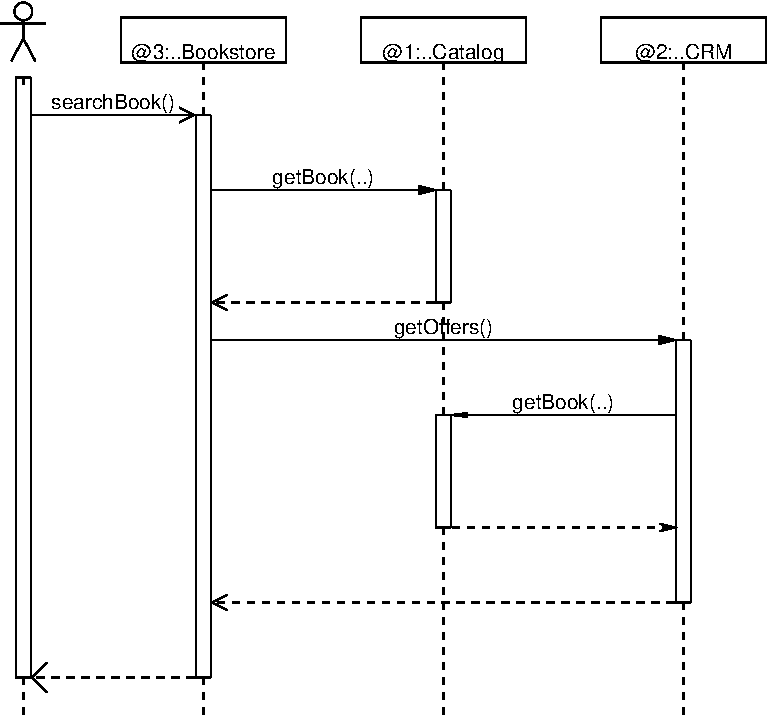
\includegraphics[scale=0.4]{images/example-plots/assemblySequenceDiagram-6488138950668976129-crop}
\caption{\textit{Assembly-level} sequence diagram of trace \ldots{}6129}
\label{fig:appendix:traceAnalysisExample:SeqDiagrDepl6129}
\end{figure}

\section{Call Trees}\label{sec:example:callTrees}%

\subsection{Trace Call Trees}\label{sec:example:traceCallTrees}%

Trace call trees are generated using the command-line option \OPT{\OPTplotCallTrees}. %
Figures~\ref{fig:appendix:traceAnalysisExample:TraceCallTrees6129}--\ref{fig:appendix:traceAnalysisExample:TraceCallTrees6141} %
show these call trees for each deployment-level %
trace equivalence representative (Section~\ref{sec:example:traceEquivClasses}).

\begin{figure}[h]\centering
\subfigure[Trace \ldots{}6129]{\label{fig:appendix:traceAnalysisExample:TraceCallTrees6129}%
\ \ 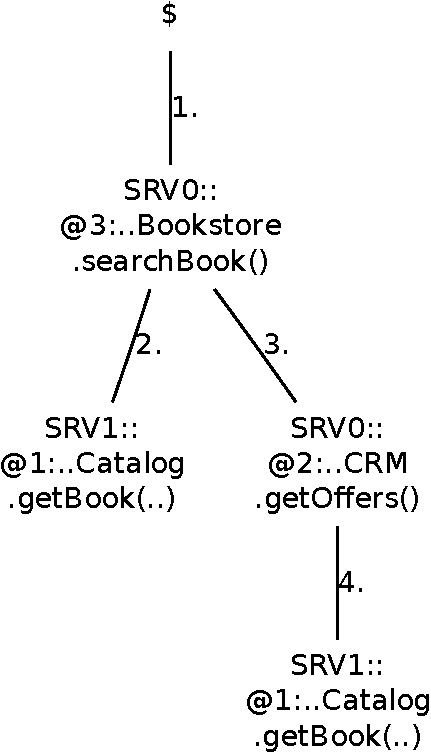
\includegraphics[scale=0.4]{images/example-plots/callTree-6488138950668976129-crop}\ \ 
}
\subfigure[Trace \ldots{}6130]{\label{fig:appendix:traceAnalysisExample:TraceCallTrees6130}%
\ \ 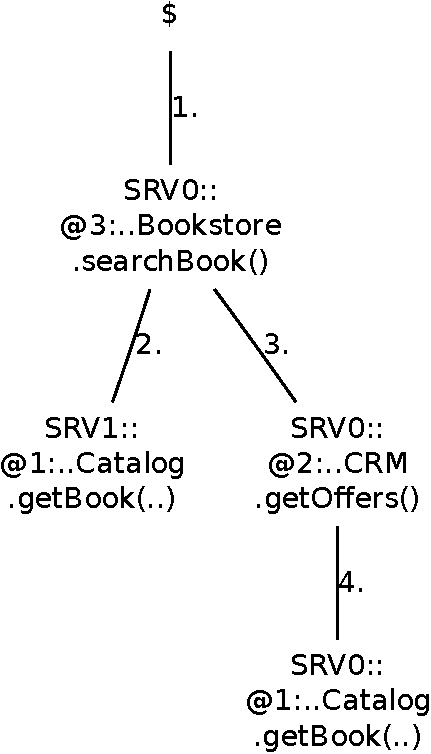
\includegraphics[scale=0.4]{images/example-plots/callTree-6488138950668976130-crop}\ \ 
}
\subfigure[Trace \ldots{}6131]{\label{fig:appendix:traceAnalysisExample:TraceCallTrees6131}%
\ \ 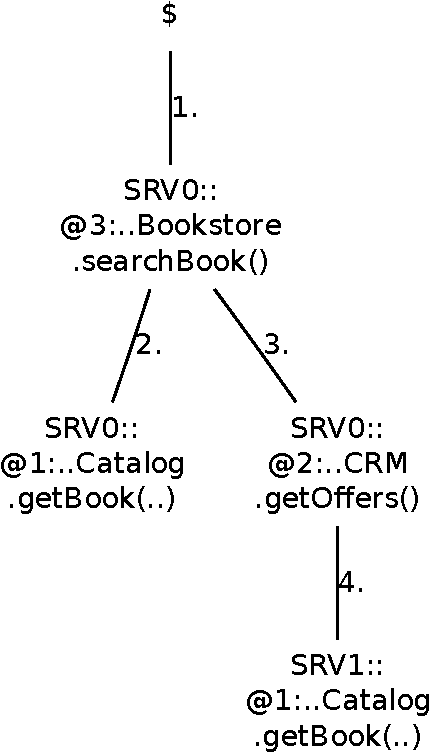
\includegraphics[scale=0.4]{images/example-plots/callTree-6488138950668976131-crop}\ \ 
}
\subfigure[Trace \ldots{}6141]{\label{fig:appendix:traceAnalysisExample:TraceCallTrees6141}%
\ \ 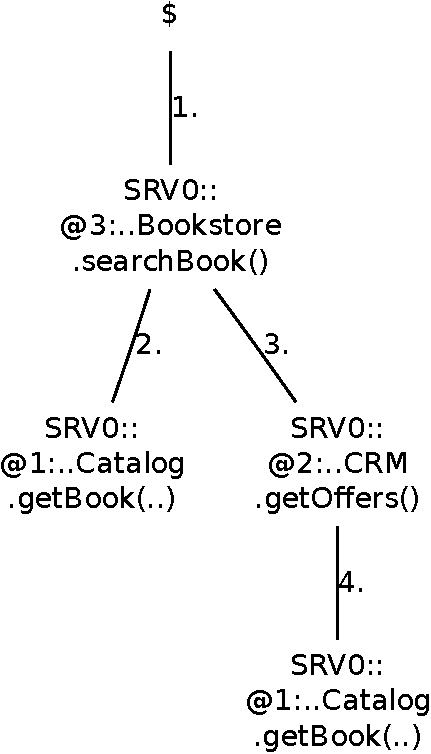
\includegraphics[scale=0.4]{images/example-plots/callTree-6488138950668976141-crop}\ \ 
}
\caption{Calls trees of the trace %
equivalence class representatives (Listing~\ref{lst:appendix:traceAnalysisExample:traceAssemblyEquivClasses})}
\label{fig:appendix:traceAnalysisExample:TraceCallTrees}
\end{figure}

\newpage

\subsection{Aggregated Call Trees}\label{sec:example:aggregatedCallTrees}%

Aggregated deployment/assembly-level call trees are generated using the command-line options %
\OPT{\OPTplotAggregatedDeploymentCallTree} and \OPT{\OPTplotAggregatedAssemblyCallTree}. %
Figures~\ref{fig:appendix:traceAnalysisExample:AggregatedCallTreesDeployment} and \ref{fig:appendix:traceAnalysisExample:AggregatedCallTreesAssembly} %
show these aggregated call trees for the traces contained in the monitoring data %
used in this section. %

\begin{figure}[h]\centering
\subfigure[deployment-level]{\label{fig:appendix:traceAnalysisExample:AggregatedCallTreesDeployment}%
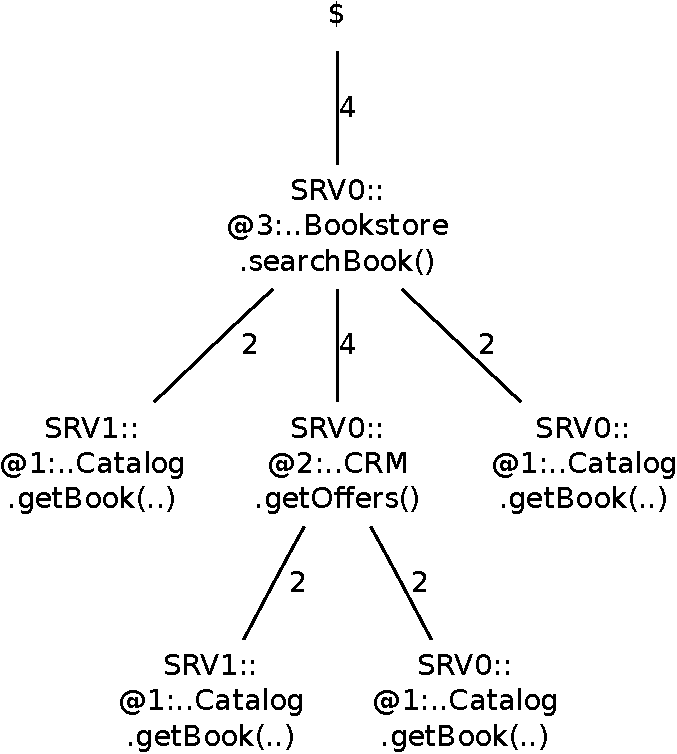
\includegraphics[scale=0.4]{images/example-plots/aggregatedDeploymentCallTree-crop}%
}
\subfigure[assembly-level]{\label{fig:appendix:traceAnalysisExample:AggregatedCallTreesAssembly}%
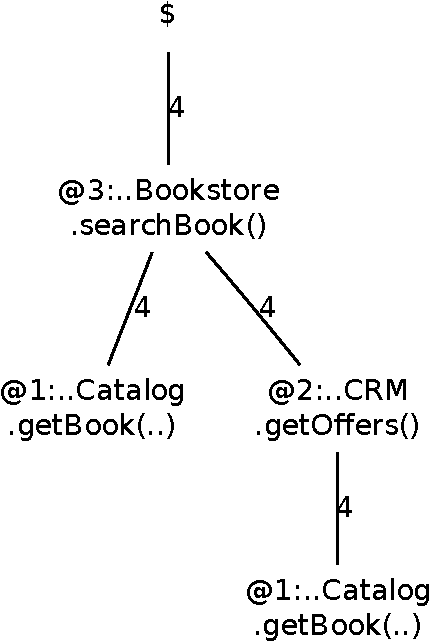
\includegraphics[scale=0.4]{images/example-plots/aggregatedAssemblyCallTree-crop}%
}
\caption{Aggregated call trees generated from the 1635~traces}
\label{fig:appendix:traceAnalysisExample:AggregatedCallTrees}
\end{figure}


\section{Dependency Graphs}

\subsection{Container Dependency Graphs}

A container dependency graph is generated using the command-line option %
\OPT{\OPTplotContainerDependencyGraph}. %
Figure~\ref{fig:appendix:traceAnalysisExample:ContainerDepGraph} shows the %
container dependency graph for the monitoring data used in this section. 

\begin{figure}[h]\centering
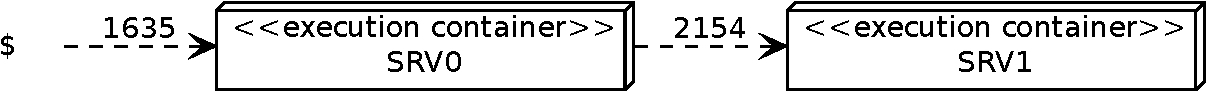
\includegraphics[scale=0.4]{images/example-plots/containerDependencyGraph-crop}
\caption{Container dependency graph}
\label{fig:appendix:traceAnalysisExample:ContainerDepGraph}
\end{figure}

\subsection{Component Dependency Graphs}

Deployment/assembly-level component dependency graphs are generated using the %
command-line options \OPT{\OPTplotDeploymentComponentDependencyGraph} and %
\OPT{\OPTplotAssemblyComponentDependencyGraph}. %
Figures~\ref{fig:appendix:traceAnalysisExample:ComponentDepGraphsDeployment} and %
\ref{fig:appendix:traceAnalysisExample:ComponentDepGraphsAssembly} show the %
component dependency graphs for the monitoring data used in this section. 

\begin{figure}[h]\centering
\subfigure[deployment-level]{\label{fig:appendix:traceAnalysisExample:ComponentDepGraphsDeployment}%
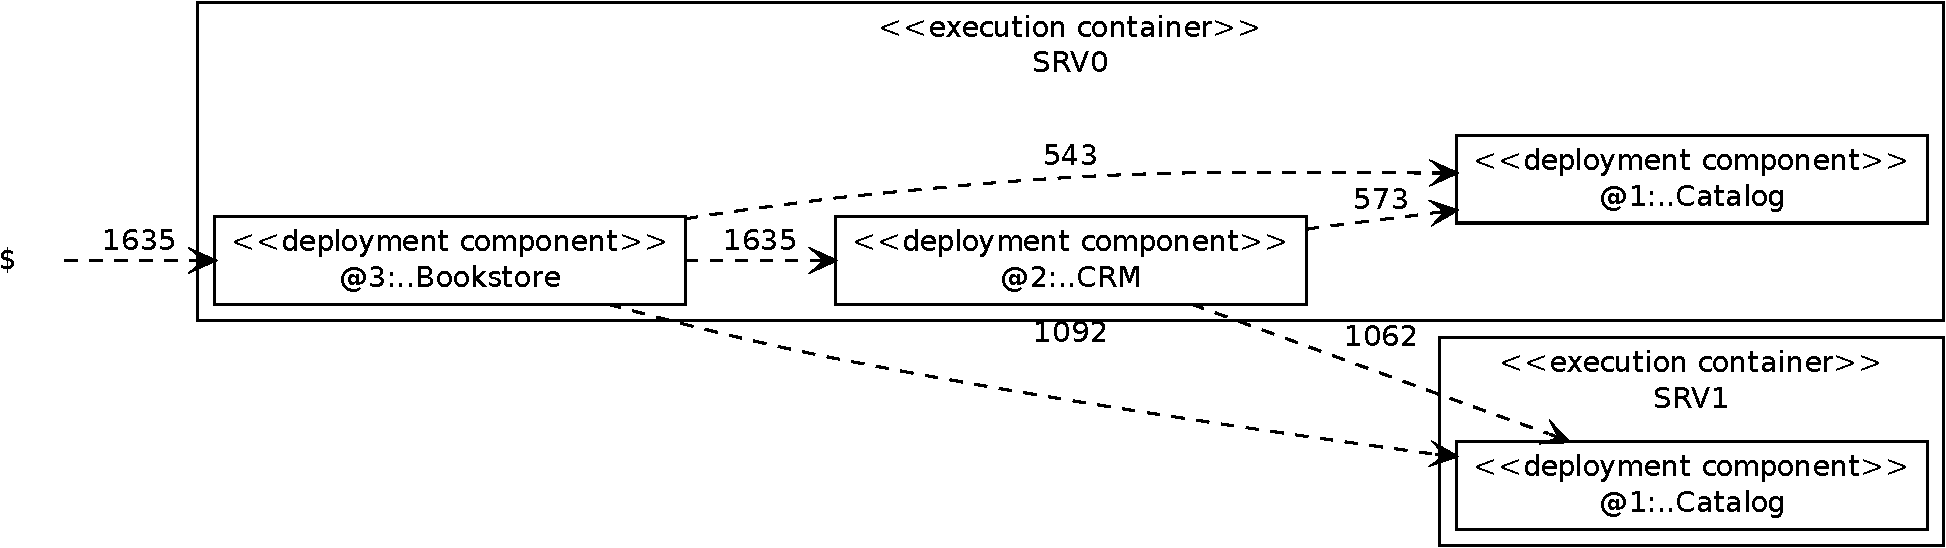
\includegraphics[scale=0.4]{images/example-plots/deploymentComponentDependencyGraph-crop}
}
\subfigure[assembly-level]{\label{fig:appendix:traceAnalysisExample:ComponentDepGraphsAssembly}%
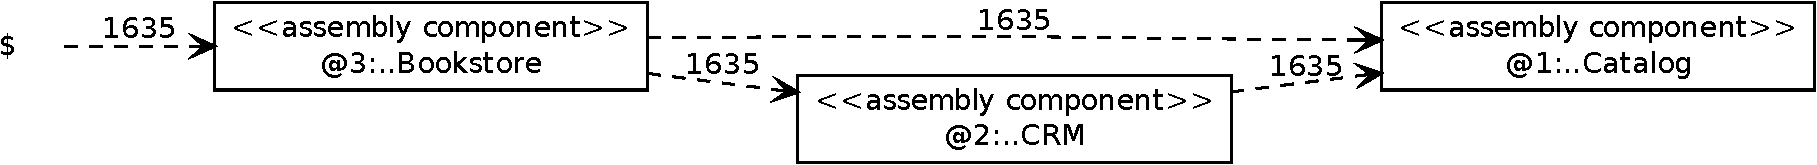
\includegraphics[scale=0.4]{images/example-plots/assemblyComponentDependencyGraph-crop}
}
\caption{Component dependency graphs}
\label{fig:appendix:traceAnalysisExample:ComponentDepGraphs}
\end{figure}

\subsection{Operation Dependency Graphs}

Deployment/assembly-level operation dependency graphs are generated using the %
command-line options \OPT{\OPTplotDeploymentOperationDependencyGraph} and %
\OPT{\OPTplotAssemblyOperationDependencyGraph}. %
Figures~\ref{fig:appendix:traceAnalysisExample:OperationDepGraphsDeployment} and %
\ref{fig:appendix:traceAnalysisExample:OperationDepGraphsAssembly} show the %
operation dependency graphs for the monitoring data used in this section. 

\begin{figure}[h]\centering
\subfigure[deployment-level]{\label{fig:appendix:traceAnalysisExample:OperationDepGraphsDeployment}%
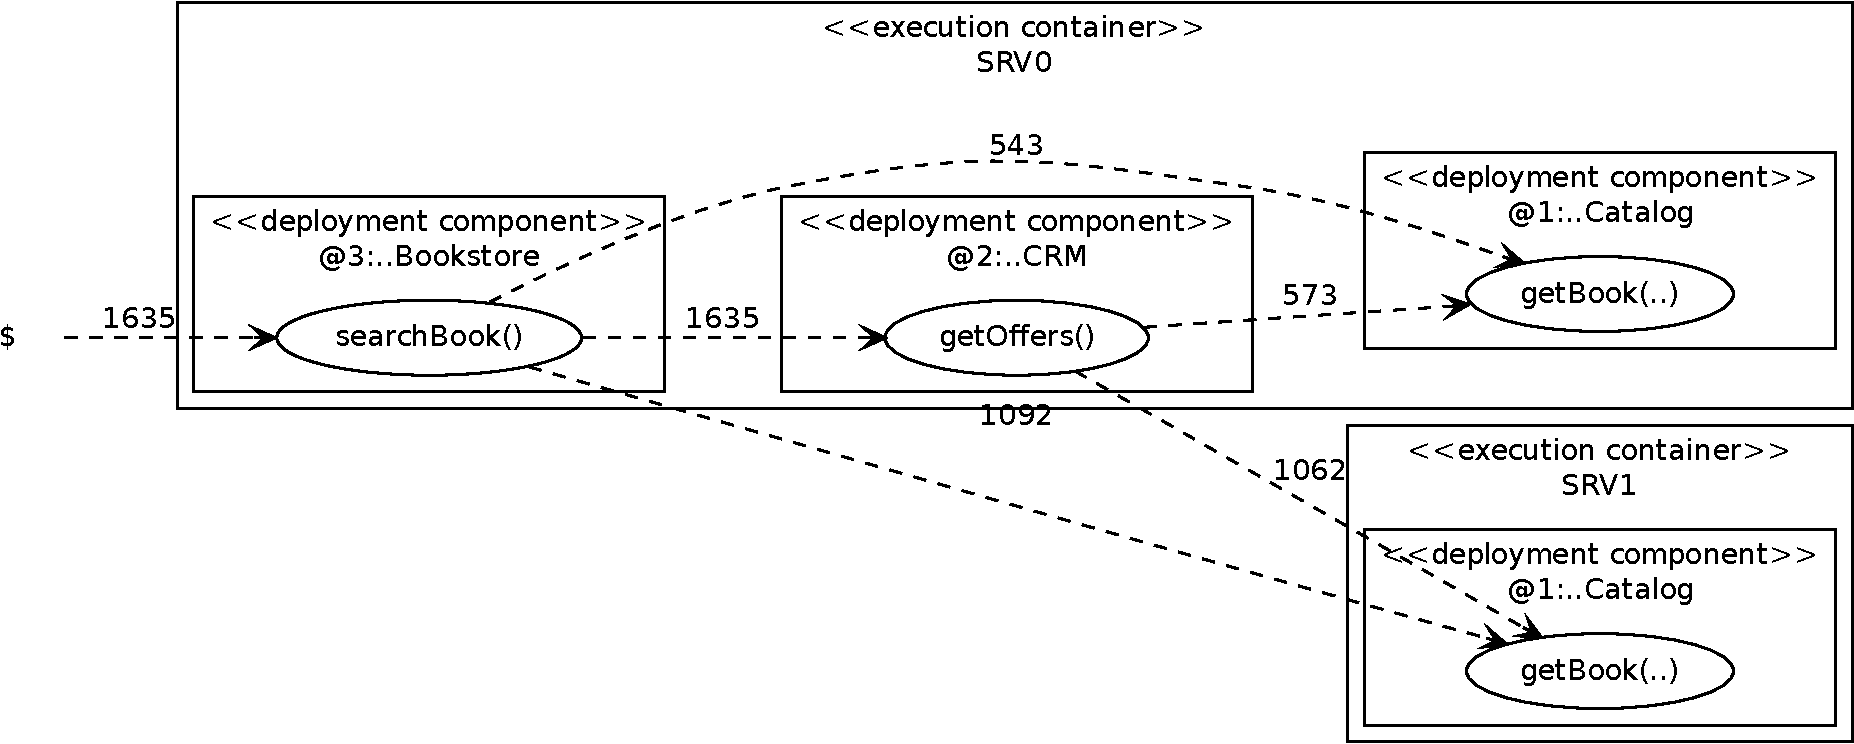
\includegraphics[scale=0.4]{images/example-plots/deploymentOperationDependencyGraph-crop}
}
\subfigure[assembly-level]{\label{fig:appendix:traceAnalysisExample:OperationDepGraphsAssembly}%
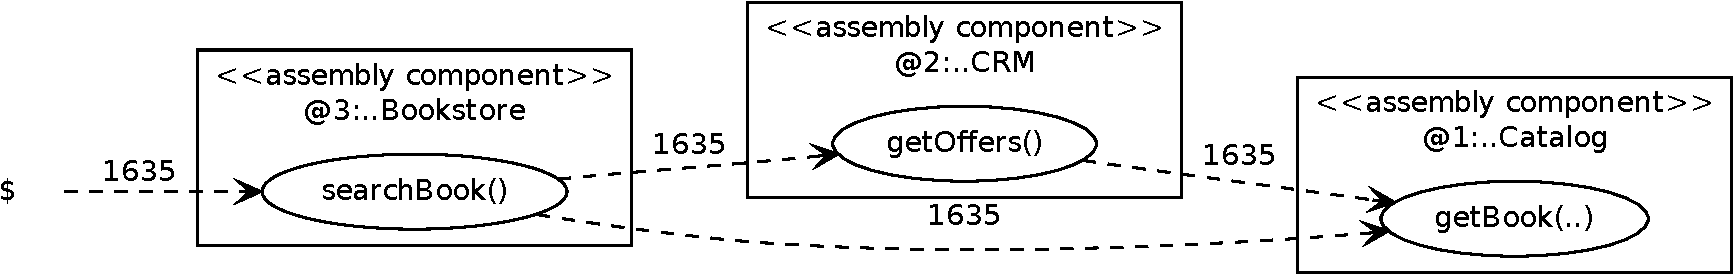
\includegraphics[scale=0.4]{images/example-plots/assemblyOperationDependencyGraph-crop}
}
\caption{Operation dependency graphs}
\label{fig:appendix:traceAnalysisExample:OperationDepGraphs}
\end{figure}

\section{HTML Output of the System Model}

\KiekerTraceAnalysis{} writes an HTML representation of the system model reconstructed %
from the trace data to a file \file{system-entities.html}. %
Figure~\ref{fig:appendix:traceAnalysisExample:htmlSystemModel} shows a screenshot %
of this file as rendered by a web browser.

\begin{figure}[h]\centering
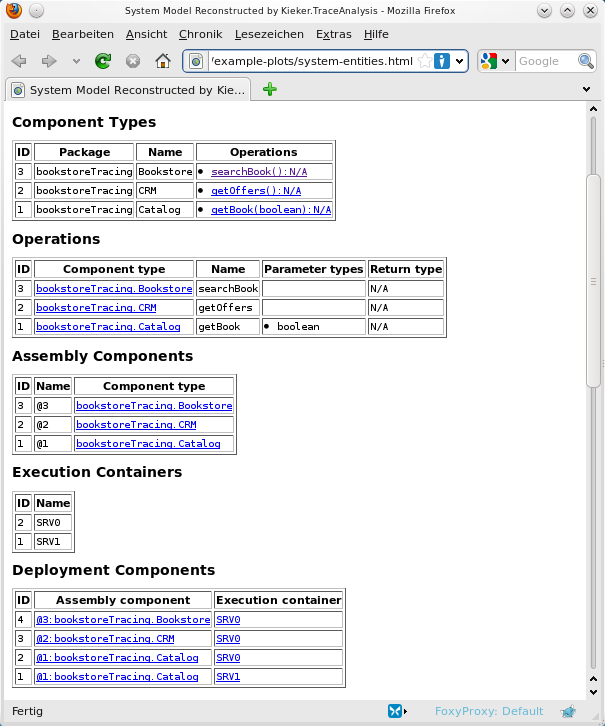
\includegraphics[width=0.6\textwidth]{images/example-plots/system-entities-html-FFscrsh.png}
\caption{HTML output of the system model reconstructed from the traces}
\label{fig:appendix:traceAnalysisExample:htmlSystemModel}
\end{figure}


% \enlargethispage{2cm}
% 	\begin{figure}[H]\centering
% 	\subfigure[deployment level]{\label{fig:appendix:allocationSequenceDiagram}
% 	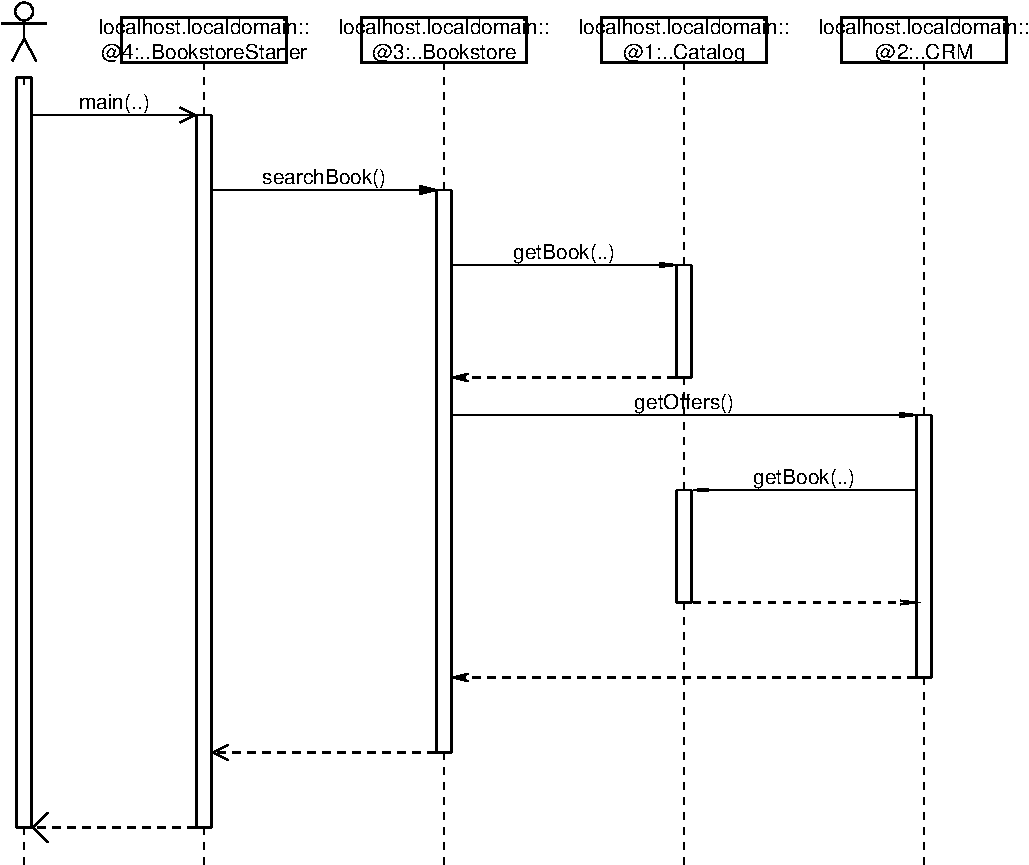
\includegraphics[scale=0.4]{images/allocationSequenceDiagram-crop}
% 	}
% 	\subfigure[assembly level]{\label{fig:appendix:assemblySequenceDiagram}
% 	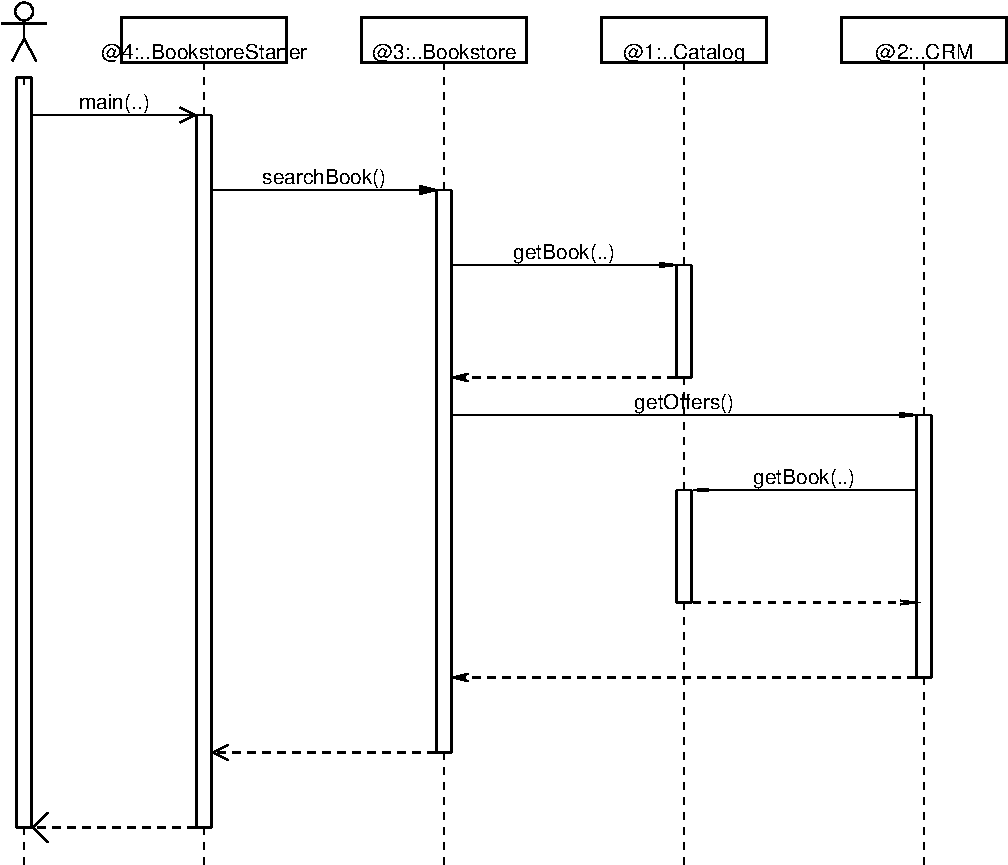
\includegraphics[scale=0.4]{images/assemblySequenceDiagram-crop}
% 	}
% 	\caption{Sequence diagrams}
% 	\end{figure}
% 
%     \begin{figure}[H]\centering
% 	\subfigure[single trace]{\label{fig:appendix:callTree}%
% 	\quad 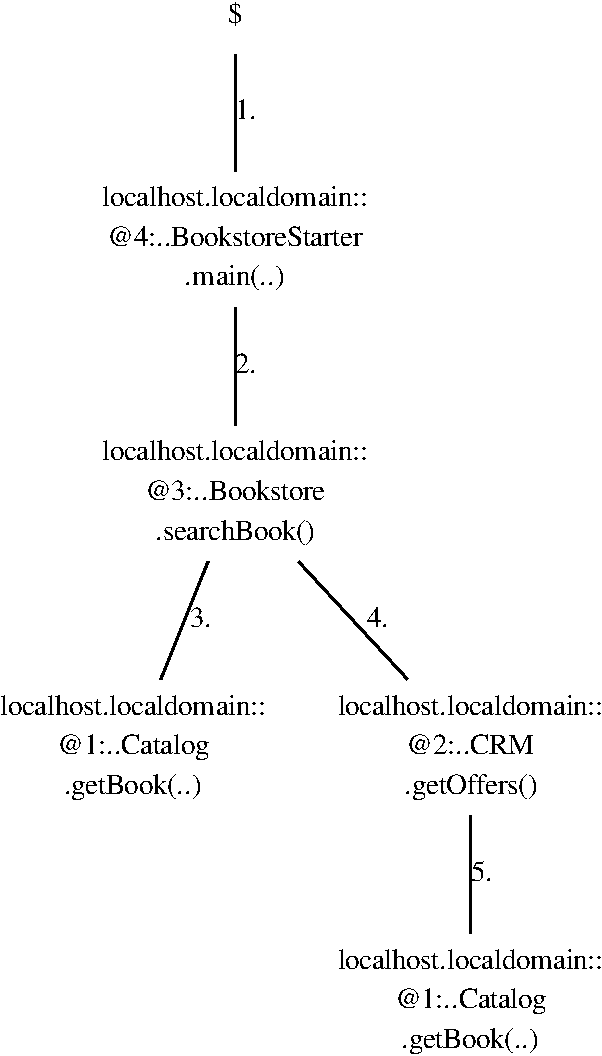
\includegraphics[scale=0.4]{images/callTree-crop} \quad%
% 	}%
% 	\subfigure[aggregated (deployment level)]{\label{fig:appendix:aggregatedAllocationCallTree}%
% 	\quad\quad 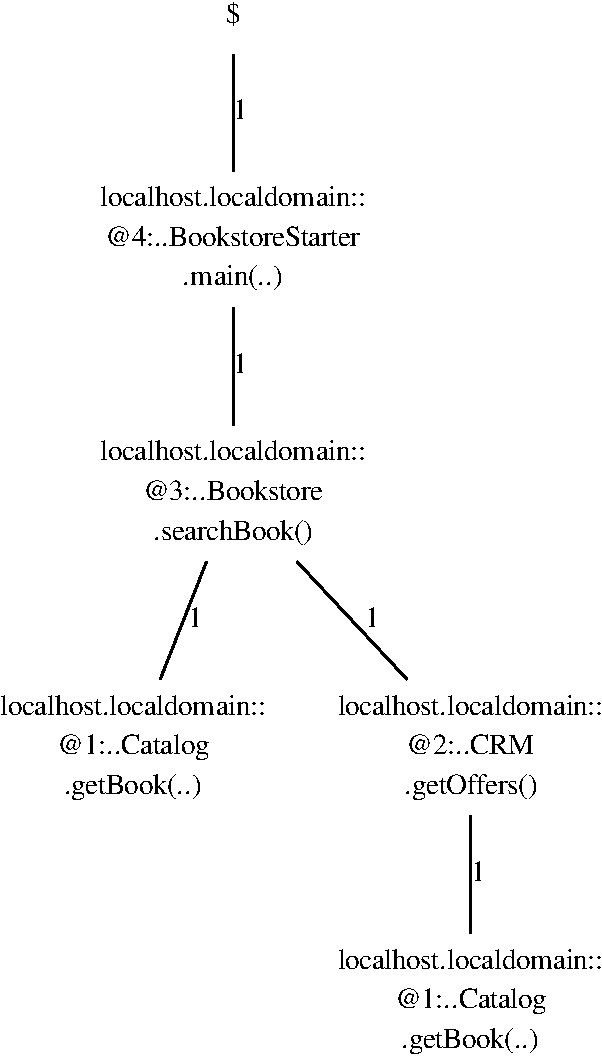
\includegraphics[scale=0.4]{images/aggregatedAllocationCallTree-crop}\quad\quad %
% 	}%
% 	\subfigure[aggregated (assembly level)]{\label{fig:appendix:aggregatedAssemblyCallTree}%
% 	\quad\quad\quad 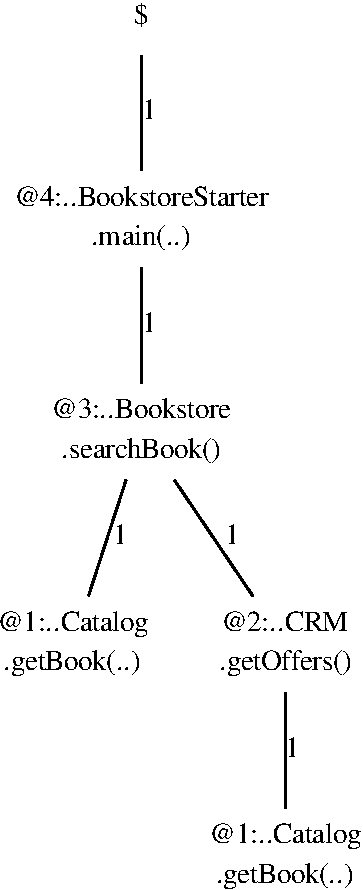
\includegraphics[scale=0.4]{images/aggregatedAssemblyCallTree-crop}\quad\quad\quad %
% 	}%
% 	\caption{Calls trees for a single trace~\subref{fig:appendix:callTree} and aggregated call %
% 	trees~\subref{fig:appendix:aggregatedAllocationCallTree}/\subref{fig:appendix:aggregatedAssemblyCallTree}}
% 	\end{figure}
% 
% \newpage
% 
% 	\begin{figure}[H]
% 		\centering
% 		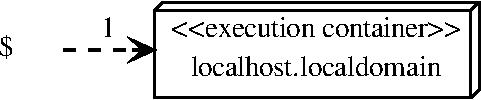
\includegraphics[scale=0.45]{images/containerDependencyGraph-crop}
% 		\caption{Container Dependency Graph}
% 	\end{figure}  
% 
%     \begin{figure}[H]\centering
% \subfigure[deployment level]{\label{fig:appendix:allocationComponentDependencyGraph}%
% 		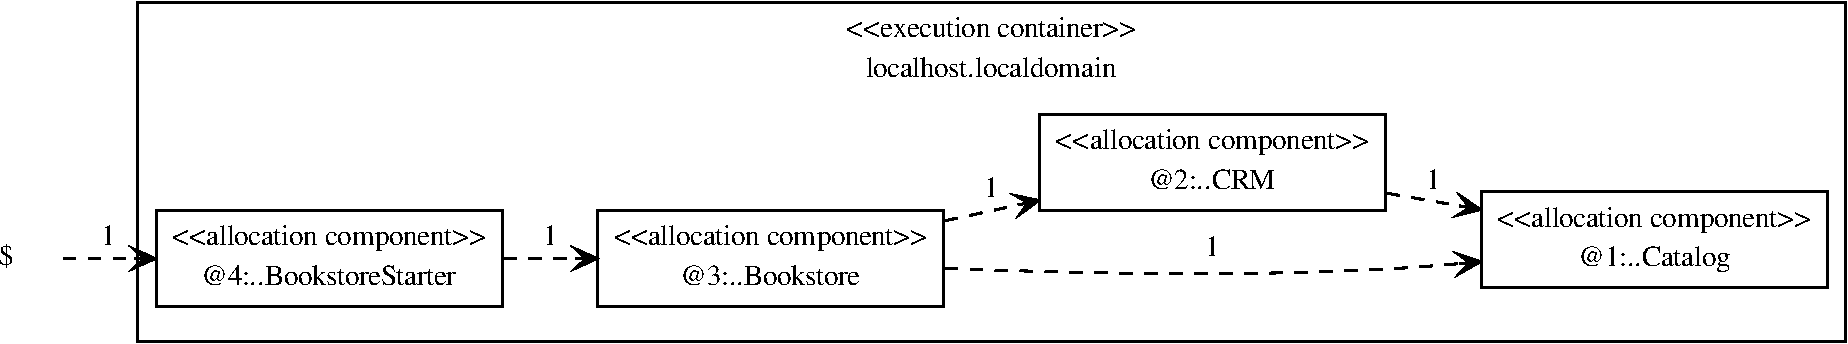
\includegraphics[scale=0.45]{images/allocationComponentDependencyGraph-crop}
% 	}\\
% 	\subfigure[assembly level]{\label{fig:appendix:assemblyComponentDependencyGraph}%
% 		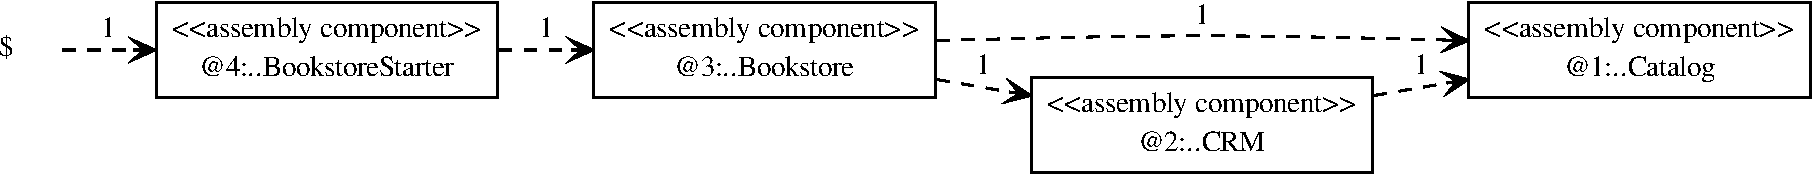
\includegraphics[scale=0.45]{images/assemblyComponentDependencyGraph-crop}
% 	}%
% 	\caption{Component Dependency Graphs}
% 	\end{figure}
% 
% 	\begin{figure}[H]\centering
% 	\subfigure[deployment level]{\label{fig:appendix:allocationOperationDependencyGraph}%
% 		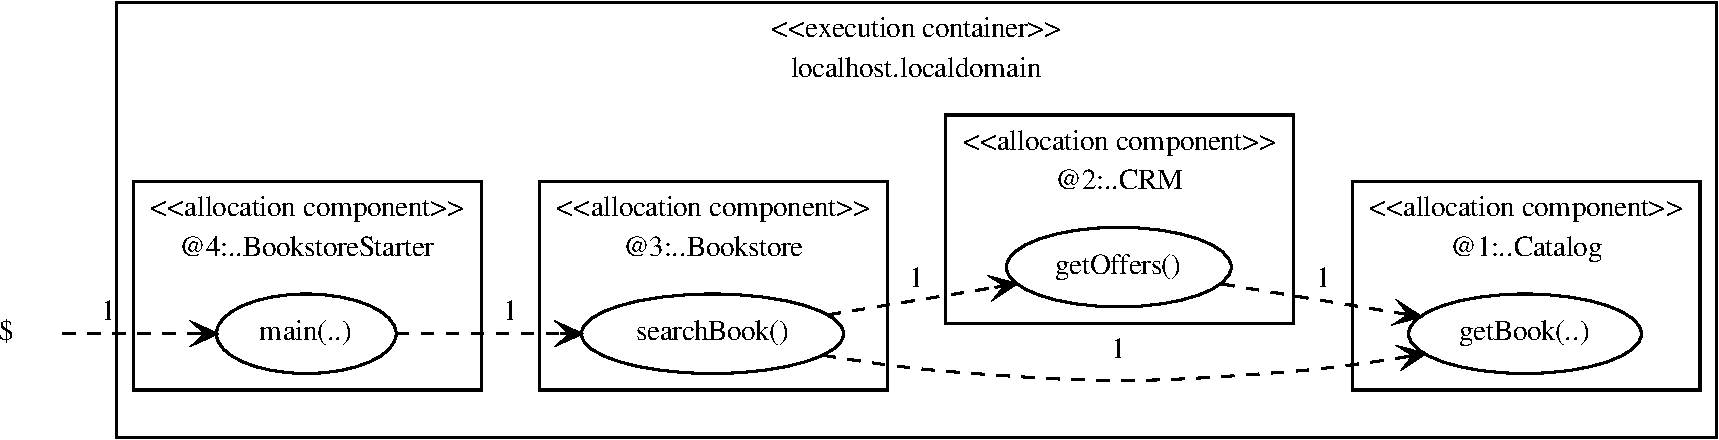
\includegraphics[scale=0.45]{images/allocationOperationDependencyGraph-crop}
% 	}\\
% 	\subfigure[assembly level]{\label{fig:appendix:assemblyOperationDependencyGraph}%
% 		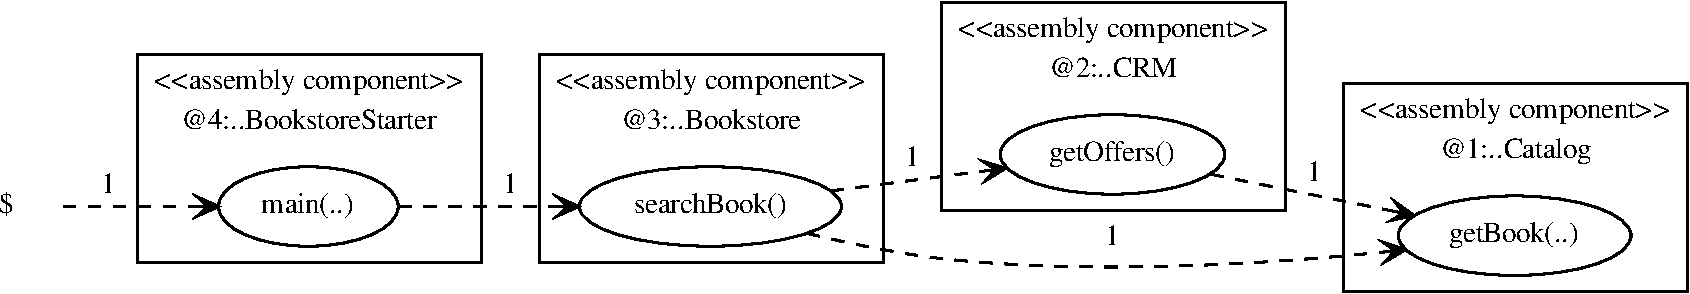
\includegraphics[scale=0.45]{images/assemblyOperationDependencyGraph-crop}
% 	}%
% 	\caption{Operation Dependency Graphs}
% 	\end{figure}